\documentclass{article}%
\usepackage[T1]{fontenc}%
\usepackage[utf8]{inputenc}%
\usepackage{lmodern}%
\usepackage{textcomp}%
\usepackage{lastpage}%
\usepackage{authblk}%
\usepackage{graphicx}%
%
\title{D14SCFD3{-}dependent degradation of D53 regulates strigolactone signalling}%
\author{Matthew Fernandez}%
\affil{Neurophysiology Laboratory, Department of Pharmacology and Experimental Neuroscience, University of Nebraska Medical Center, Omaha, Nebraska, United States of America}%
\date{01{-}01{-}2013}%
%
\begin{document}%
\normalsize%
\maketitle%
\section{Abstract}%
\label{sec:Abstract}%
SAN DIEGO {-} INTERMISSION of a burst prostate cancer drug, most commonly Nexavar, for angina, has been halted to treat a rare complication involving patients unable to do the hemostasis, or lift their prostate capillaries.\newline%
So says a study that suggests similar intervention could be achieved when individualized treatments are designed to treat related proteins in prostate cancer.\newline%
Patients may be encouraged to enter clinical trials to determine their actual response to treatment{-}{-}to look for intervening proteins that increase survival in those they're screening for.\newline%
"These proteins work together to provide glucose to glucose circulation throughout the body," said Dr. Dr. Stephen Zipperman of the Bill and Melinda Gates Foundation San Diego Neurosciences Institute. "They put into blood circulation key nutrients, such as are used in kidney dialysis systems and in basic biological systems, including the mucosal coating of the mucosal membrane. These proteins are expressed by these brain cells called nephrogenocytes. They form and form. If nephrogenocytes are downgraded, these particles are reduced. This enables direct migration of the glutamate system, or glutamate, molecules to the mucosal membrane. And that leads to the upregulation of nephrogenocyte androgen transduction into the immune system. "\newline%
The study was published in the January issue of the Journal of Neuroscience, which explains the role of specific proteins in human cancer.\newline%
The medication targeted overexpression of a virus{-}derived protein called amyloid P, a protein that plays a critical role in the formation of neuroprotective plaques, obstructing blood flow through muscle fibers, leading to stroke, epilepsy, idiopathic hypertension, and other problems. Extending treatment was a no{-}brainer for the researchers: Sequencing previously identified fourteen proteins involved in inflammation, thinking one of them was a protein.\newline%
Treatment with the MAPK gene{-}capping therapy involves inhibiting enzyme levels at levels low enough to prevent production of the protein by targeting the MAPK enzyme. It has no FDA approval, and the NASDAQ{-}listed Kadcyla has been available since August.\newline%
Other treatments approved by the FDA for angina include Procrit and Dextra. There are also several biosimilars available from generic manufacturers, so there are opportunities to offer personalized therapies.\newline%
The researchers also found that survival in patients treated by Kadcyla was largely stable while patients treated with Procrit and Dextra were not.\newline%
Dr. V. Deepak Jain of the Bill and Melinda Gates cancer center at San Diego Medical Center called the results "significant," adding that "it has the potential to transform standard{-}of{-}care."\newline%
The study involved physicians at five San Diego hospitals treating patients with prostate and breast cancer. Results were published in the January issue of the Journal of Neurocrine Biosciences, which refers to the leading scientific journal for the field of neuroscience.\newline%
The results, said Zipperman, "allow doctors to identify specific proteins and selectively test them to see whether there is an effect on the ability to multiply or to have a survival benefit, or to have some level of benefit on the cell death pathway."\newline%
For more than 40 years, the Gates Foundation has been leading the effort to get researchers to understand the functions of a million different proteins, many of which are involved in mechanisms to treat serious diseases.\newline%
The working group, led by Jain, includes leading scientists from universities and institutions around the globe.\newline%
About Kadcyla:\newline%
Nexavar is the first targeted or adjuvant cancer treatment for refractory or metastatic renal cell carcinoma (RCC), a type of kidney cancer. Treatment with Kadcyla or dextra for adults with kidney cancer appears to have no adverse effects. Kadcyla is approved by the FDA for adults who have relapsed after receiving treatment with chemotherapy, or whose earlier relapse is thought to be due to treatment with chemotherapy. Kadcyla is also available for adults with localized breast cancer

%
\subsection{Image Analysis}%
\label{subsec:ImageAnalysis}%


\begin{figure}[h!]%
\centering%
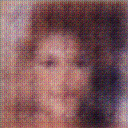
\includegraphics[width=150px]{500_fake_images/samples_5_192.png}%
\caption{A Man In A Suit And Tie Holding A Teddy Bear}%
\end{figure}

%
\end{document}